\begin{figure}[htbp]
\section*{ FBN1}
\centering
\begin{subfigure}[b]{0.65\textwidth}
\centering
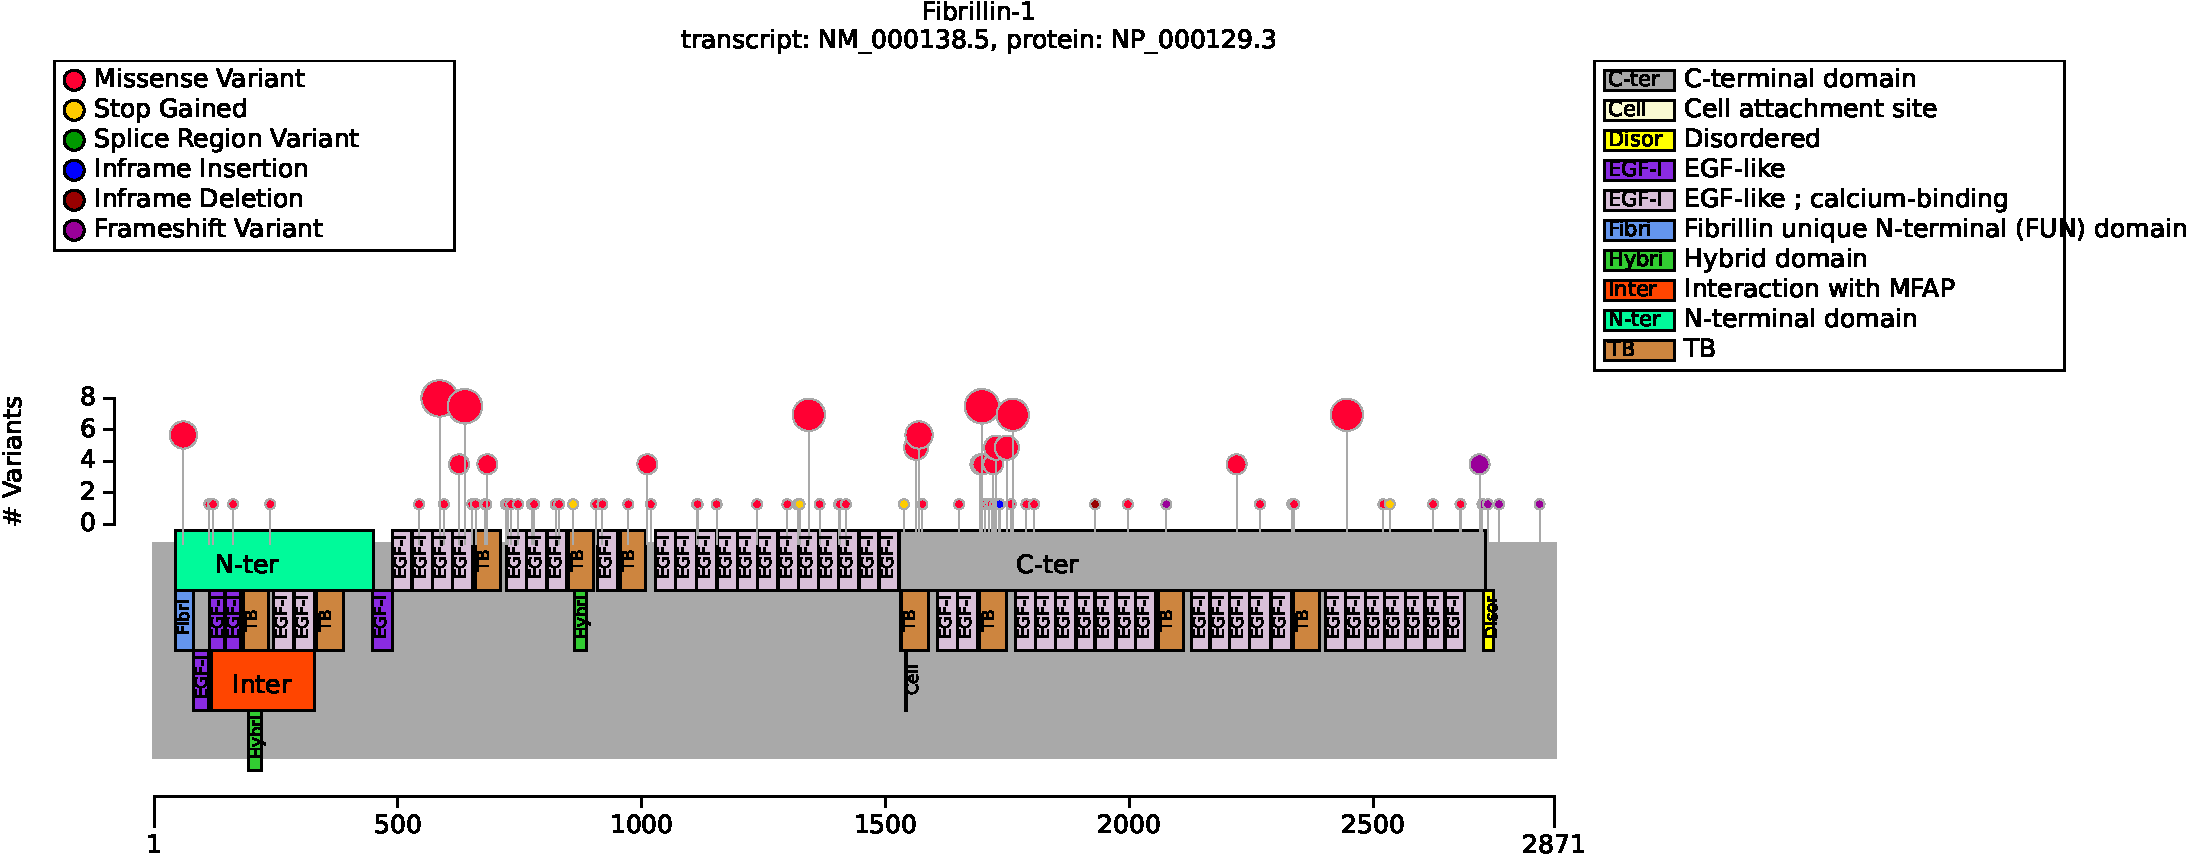
\includegraphics[width=\textwidth]{ img/FBN1_protein_diagram.pdf} 
\captionsetup{justification=raggedright,singlelinecheck=false}
\caption{Distribution of variants in FBN1}
\end{subfigure}


\begin{subfigure}[b]{0.95\textwidth}
\centering
\resizebox{\textwidth}{!}{
\begin{tabular}{llllrr}
\toprule
HPO term & missense & other & p-value & adj. p-value\\
\midrule
Arachnodactyly [HP:0001166] & 34/81 (42\%) & 18/22 (82\%) & 0.001 & 0.026\\
Thoracic aortic aneurysm [HP:0012727] & 25/64 (39\%) & 12/14 (86\%) & 0.002 & 0.026\\
Hyperextensibility of the finger joints [HP:0001187] & 0/78 (0\%) & 3/14 (21\%) & 0.003 & 0.026\\
\bottomrule
\end{tabular}
}
\captionsetup{justification=raggedright,singlelinecheck=false}
\caption{Fisher Exact Test: missense vs. other. Total of 27 tests were performed. }
\end{subfigure}
\begin{subfigure}[b]{0.95\textwidth}
\centering
\resizebox{\textwidth}{!}{
\begin{tabular}{llllrr}
\toprule
HPO term & TB domain & cbEGF & p-value & adj. p-value\\
\midrule
Ectopia lentis [HP:0001083] & 9/18 (50\%) & 48/59 (81\%) & 0.013 & 0.038\\
Mitral valve prolapse [HP:0001634] & 1/28 (4\%) & 13/47 (28\%) & 0.012 & 0.038\\
Disproportionate tall stature [HP:0001519] & 2/40 (5\%) & 12/43 (28\%) & 0.007 & 0.029\\
Tall stature [HP:0000098] & 7/38 (18\%) & 21/40 (52\%) & 0.002 & 0.011\\
Severe short stature [HP:0003510] & 15/36 (42\%) & 0/24 (0\%) & $1.36\times 10^{-4}$ & $9.04\times 10^{-4}$\\
Proportionate short stature [HP:0003508] & 20/36 (56\%) & 0/24 (0\%) & $2.35\times 10^{-6}$ & $2.35\times 10^{-5}$\\
Short stature [HP:0004322] & 23/39 (59\%) & 0/24 (0\%) & $4.39\times 10^{-7}$ & $8.79\times 10^{-6}$\\
\bottomrule
\end{tabular}
}
\captionsetup{justification=raggedright,singlelinecheck=false}
\caption{Fisher Exact Test: TB domain vs cbEGF. Total of 20 tests were performed. }
\end{subfigure}

\begin{subfigure}[b]{0.95\textwidth}
\centering
\resizebox{\textwidth}{!}{
\begin{tabular}{llllrr}
\toprule
HPO term & exon 37 & other & p-value & adj. p-value\\
\midrule
Arachnodactyly [HP:0001166] & 0/8 (0\%) & 52/95 (55\%) & 0.003 & 0.019\\
Ectopia lentis [HP:0001083] & 1/9 (11\%) & 78/100 (78\%) & $1.12\times 10^{-4}$ & 0.001\\
Stiff skin [HP:0030053] & 8/9 (89\%) & 0/50 (0\%) & $4.06\times 10^{-9}$ & $8.52\times 10^{-8}$\\
\bottomrule
\end{tabular}
}
\captionsetup{justification=raggedright,singlelinecheck=false}
\caption{Fisher Exact Test:  exon 37 vs. other. Total of 21 tests were performed. }
\end{subfigure}
\begin{subfigure}[b]{0.95\textwidth}
\centering
\resizebox{\textwidth}{!}{
\begin{tabular}{llllrr}
\toprule
HPO term & fs last two & other & p-value & adj. p-value\\
\midrule
Hyperextensibility of the finger joints [HP:0001187] & 2/2 (100\%) & 1/90 (1\%) & $7.17\times 10^{-4}$ & 0.012\\
\bottomrule
\end{tabular}
}
\captionsetup{justification=raggedright,singlelinecheck=false}
\caption{Fisher Exact Test: Frameshift in last two exons vs other. Total of  12 tests were performed. }
\end{subfigure}
\caption{The cohort comprised 144 individuals (57 females, 55 males, 32 with unknown sex). 
4 of these individuals were reported to be deceased. A total of 109 HPO terms were used to annotate the cohort. 
Numerous articles on genotype-phenotype correlations have been published \cite{PMID_29357934,PMID_33731877,PMID_33174221}, 
but the available data is said to be be imprecise and incomplete \cite{PMID_27906200} and many studies only share aggregate data.
Disease diagnoses: Marfan syndrome (n=51), Ectopia lentis, familial (n=44), Geleophysic dysplasia 2 (n=19), 
Acromicric dysplasia  (n=13), Marfan lipodystrophy syndrome (OMIM:616914) (n=9), Stiff skin syndrome  (n=8).  
A total of 94 unique variant alleles were found in \textit{FBN1} (transcript: \texttt{NM\_000138.5}, protein id: \texttt{NP\_000129.3}).}
\end{figure}
